


\chapter{ Experimental Setup}

\section{Thomas Jefferson Lab}
\paragraph{}Thomas Jefferson Lab (Jlab) in Newport News, Virgina hosted the MARATHON experiment in the Fall of 2017. Jlab uses support from the U.S. Department of Energy(DOE) and the state of Virgina to complete the lab's mission of delivering productive research by exploring the atomic nucleus and its fundamental constituents, including precise tests of their interactions. Along with applying an advanced particle accelerator, particle detectors and other technologies to develop new basic research capabilities and to address the challenges of a modern society.
	\subsection{CEBAF}
	\paragraph{}The Continuous Electron Beam Accelerator Facility (CEBAF) was recently upgraded to a 12 GeV accelerator, upgrading it to be able to supply a 11 GeV beam of continuous electrons of up to 200 $\mu$A of current. to three experimental halls (A,B,C) and 12 GeV to the recently constructed hall D. After being accelerated to 45 MeV by a polarized electron gun or a thermionic injector, the electrons are injected into the North linear accelerator (LINAC), shown in figure \ref{CEBAF}. The polarized gun can supply electrons with up to 80$\%$ polarization and the polarization direction can be controlled by a wien filter. To ensure the level of polarization, a 5 MeV Mott polarimeter may be used to measure the level of polarization\cite{HallA}.
	\paragraph{} The electrons are conveyed through two LINACs and two bending arcs per complete pass of the accelerator. Electrons traveling to Halls A, B, and C complete a maximum of four and a half revolutions around the accelerator. Electrons going to all D travel through the north LINAC for an extra boost. These particles receive approximately 2.2 GeV in energy for each cycle through the accelerator. The radio frequency (RF) cavities in each LINAC use an oscillating electromagnetic field to supply a force to accelerate the passing electrons. These Niobium RF cavities are cooled to 2 K in order to create conditions that allow the cavities to be superconducting \cite{HallA}.    
	
	\begin{figure}[h]
	\centering
	 \caption{Schematic Layout of CEBAF. }
	 \label{CEBAF}
	 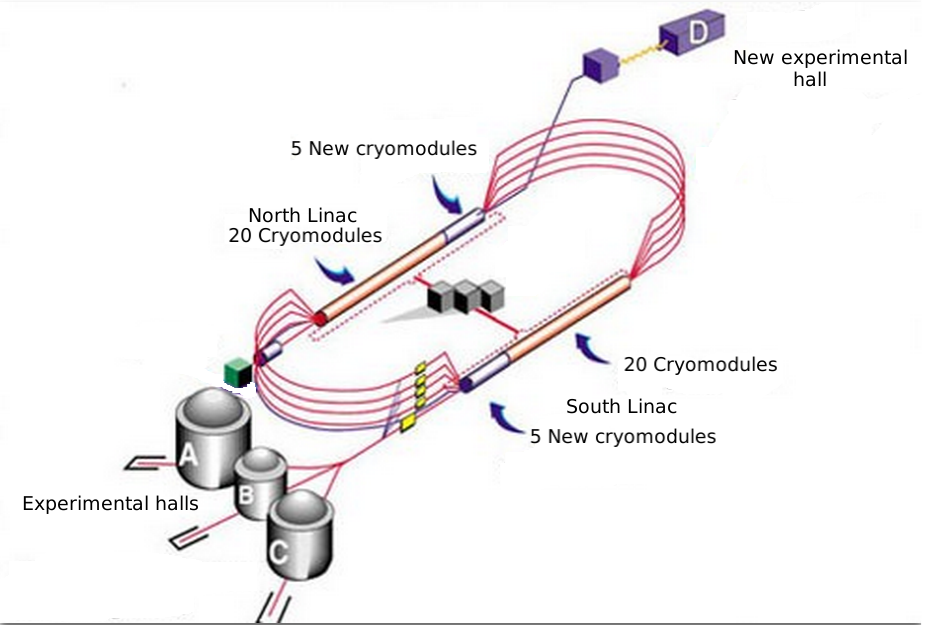
\includegraphics[width=10cm]{CEBAF.png} 
	 \end{figure} 
	 
	 \subsection{Hall A}
	 
	\begin{figure}[H]
		\centering
		\caption{A 3D drawing of Hall A. }
		\label{HallA}
		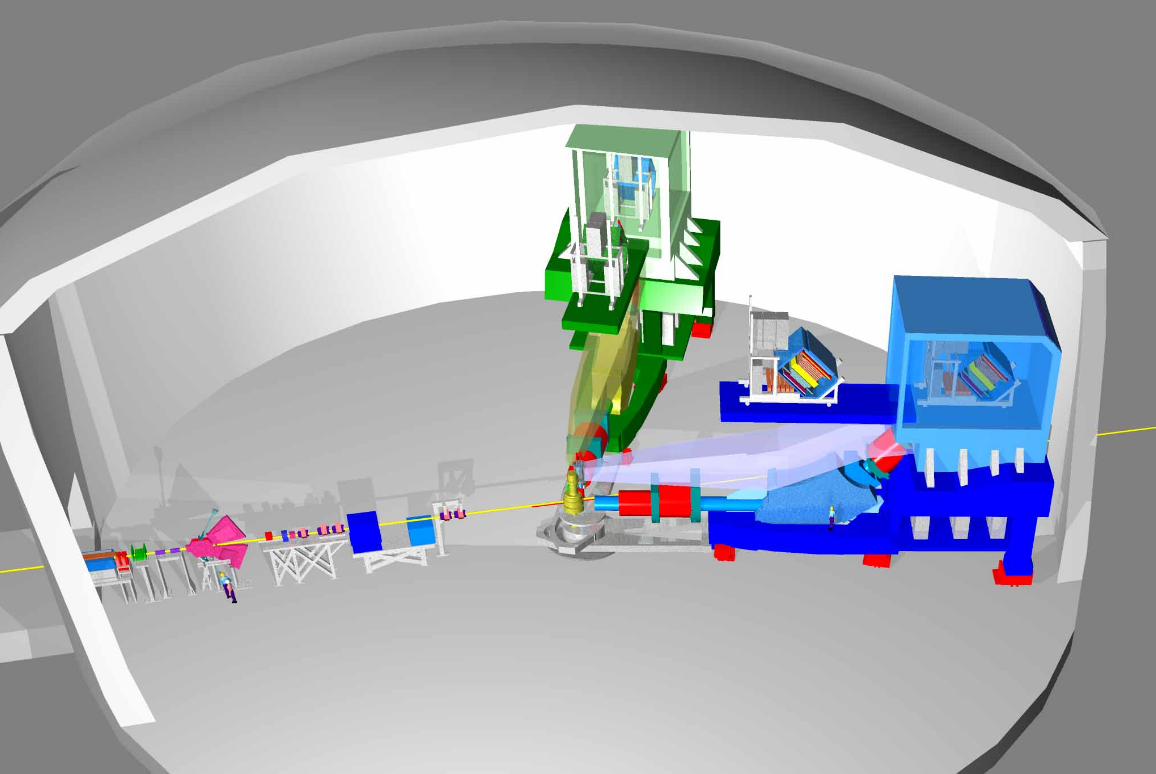
\includegraphics[width=14cm]{HallA_2.png} 
	\end{figure} 	 
	 
	 \paragraph{}The experimental Hall A and the scientific equipment used were designed for detailed investigations of the internal structure of nuclei. Two high resolution spectrometers in Hall A use the inclusive (e,e$\prime$) and exclusive (e,e$\prime$ p) reactions to gain a greater understanding of the structure of the nucleus. Completing detailed studies with high resolution and extreme accuracy requires knowing the beam position, size, energy, current, direction, and polarization when the beam strikes the target. The instrumentation used in the precise measurement of these quantities in Hall A  are shown in figure \ref{BeamLine} \cite{HallA}.

	 \paragraph{} A pair of Beam Position Monitors(BPMs) are used to measure the relative beam position without affecting the beam. The two Hall A BPMs are located at 7.524 m and 1.286 m away from the target. Using the standard difference-over-sum technique, the relative beam position is determined with an accuracy of 100 $\mu$m with a beam current of at least 1 $\mu$A \cite{HallA}. The BPMs' positional data is recorded in two ways. Every second of beam time, the beam position average over 0.3 seconds is logged into the Experimental Physics and Industrial Control System (EPICS) database. The BPMs also transmit data event-by-event to the CEBAF online Data Acquisition system(CODA).
	 	 	 
 	 	\begin{figure}[H]
 	 		\centering
 	 		\caption{A schematic layout of the beam line in Hall. \cite{HallA} }
	 	 	\label{BeamLine}
	 	 	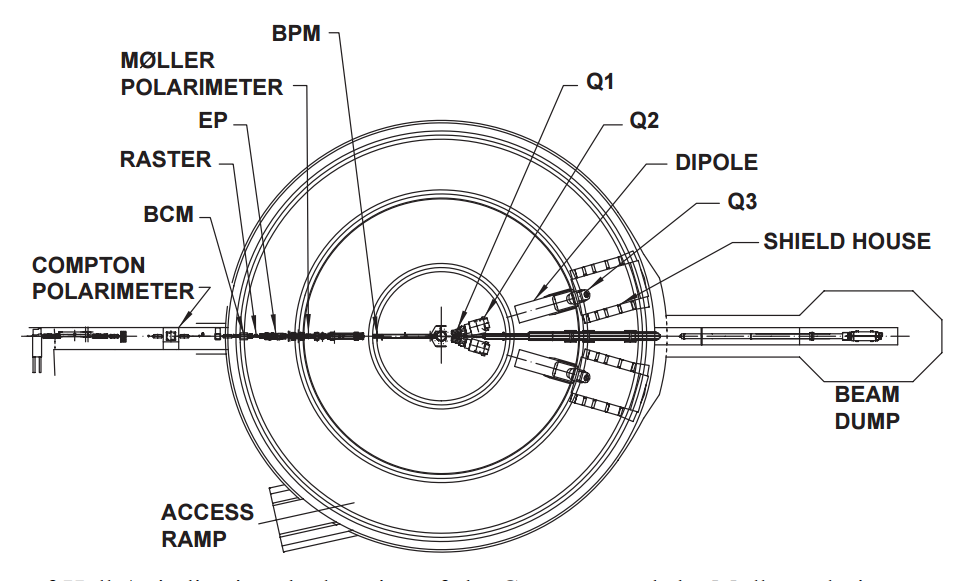
\includegraphics[width=14cm]{BeamLine.png} 
	 	 \end{figure} 	
	 	 	
	 \paragraph{} The main beam line components of the BPMs consist of four open-ended antennas. Figure \ref{BPMimg} shows a BPM chamber and figure \ref{BPM_4} shows the layout of the four antennas as you look down the beam line. In this chamber, the design of three of the four antennas can be seen. The antennas are titled $u_+$, $u_-$ and $v_+$, $v_-$. The antennas receive an induced signal as electrons pass to determine the beam position in the u and v directions. The direction of the beam is determined by using the two BPMs in conjunction with timing information provided. The accuracy of the BPMs requires an absolute measurement of the electron beam's position to calibrate the BPMs and a twiddle measurement to supply BPM signal coefficients.  \cite{BPM,BPM2}.
	 	 	\begin{figure}[H]
	 	 		\centering
	 	 		\caption{BPM design diagram, from JLab instrumentation	group. Beam direction is from left to right \cite{BPM2}. }
	 	 		\label{BPMimg}
	 	 		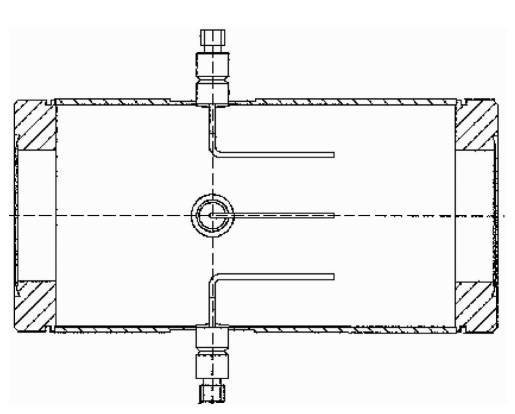
\includegraphics[width=10cm]{BPM.png} 
	 	 	\end{figure} 	
	 
	 		\begin{figure}[H]
	 			\centering
	 			\caption{BPM design diagram, looking down the beam line\cite{BPM2}. }
	 			\label{BPM_4}
	 			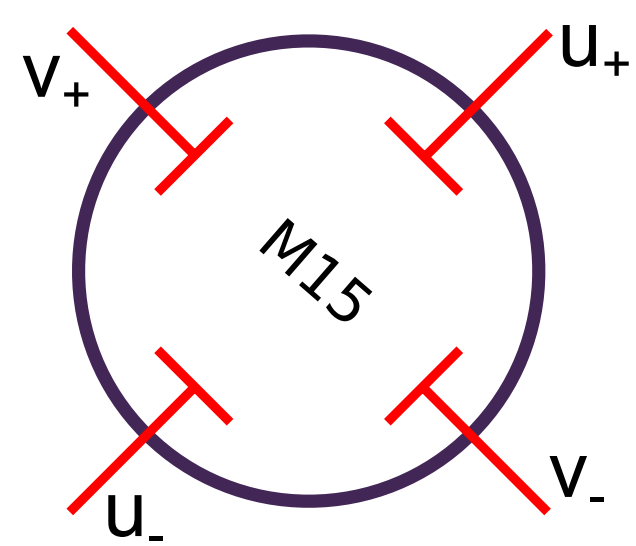
\includegraphics[width=10cm]{BPM_4.png} 
	 		\end{figure} 

	
	 \paragraph{} Damage to a target system from intense beam can cause extreme fluctuations in the target's temperature and density. A raster was used to counteract the damage caused by a focused beam. The raster used two magnetic fields produced by two dipoles to spread the electron beam out. This produces a large rectangle interaction area on the outer wall of the target. A triangle wave of 25 kHz was used to control the coils of the dipole magnets. Safety constraints administrated by the target group at JLAB limited the minimum size of the raster spot for the MARATHON experiment to two millimeters by two millimeters. The raster systems are located $\approx$17 meters before the target chamber (upstream of the target\cite{BPM2}). The rasters position can be seen in figure \ref{HallA}.  The raster changes the position of the incoming electrons based on the current supplied to the magnets used. In order to obtain the change in beam position due to the rasters activity, a raster current to beam position calibration constant was determined. 
	 
	 
	 \paragraph{}The electron beam energy is located in many of the equations used in an electron scattering experiment. This can cause a noticeable increase in systematic error if the beam energy measurement is not made precisely. At JLAB, the beam energy is measured in two ways. In Hall A, the beam energy is measured by using the (e,e$\prime$p) method. On the beam line, 17 meters upstream from the target an ep scattering chamber is located. The beam is directed into the target containing a rotating 10-30 $\mu$m thick tape of C$H_2$. The scattered angle of the electron and the recoil angle of the proton are used to determine the beam energy using equation \ref{EP}. Where $M_p$ is the mass of the proton and $\theta_p, \theta_e$ is the scattered angle of the proton, electron respectively. 
	\begin{equation}
	\label{EP}
	E = Mp \frac{cos\theta_e + \frac{sin\theta_e}{tan\theta_p}-1}{1 - cos\theta_e} 
	\end{equation}
	The beam energy was also measured using the ark measurement method \cite{Flay}. This method uses changes is beam position and precise measurements of the magnetic fields around the beam to determine the energy of the electron beam. The angle at which the electrons are bent through is related to the momentum of the electrons by the equation \ref{arc}.
	\begin{equation}
	\label{arc}
	p = k \frac{\int \vec{B} \cdot d\vec{l}}{\theta}
	\end{equation}	
	In equation \ref{arc}, p is the momentum of the electrons, $\theta$ is the bend angle, and $\vec{B}$ is the magnetic field the electron experiences. Then using the momentum of the electron, the energy of the beam can be extracted. The error on the beam energy measurement is $\delta$ E/E $\approx$ 2 $* 10^{-4} $ \cite{EPMet, Flay}.  The MARATHON experiment used both methods to accurately determine the electron beam energy.  
\section{Target}

\section{High Resolution Spectrometers}
Electrons that successfully scatter from the target may end up in the HRS(High Resolution Spectrometers). The HRSs were designed to detect charged particles with a high degree of precision. In order to achieve a high level of resolution in momentum and angle, the HRSs were designed with a magnet configuration of QQ$D_n$Q (Quadrupole, Quadrupole, Dipole, and Quadrupole). The vertical bending dipole provides the field required to transport the scattered particles through the 45$^\circ$ bending angle to the detector hut. The spectrometers were designed to perform various functions which include: triggering the data acquisition system (DAQ) when certain requirements are met, gathering the position and direction of individual particles to reconstruct a track, provide precise timing information, and identify many different particle types that pass through the detector system. Both the Left and Right HRSs contain two planes of Scintillators to function has the main trigger for the detector package. The vertical drift chambers (VDC) that lay at the front of the detector in conjunction with the Shower that lies in the back of the detector provide information for reconstructing the particle tracks and precise timing. Particles are identified by the Cherenkovs, shower calorimeters, and Pion Rejectors that are contained in the left or right HRS. The layout of the individual detectors that make up the left and right detector package are shown in figure \ref{hrsss}  \cite{HallA}.

\begin{figure}
\centering

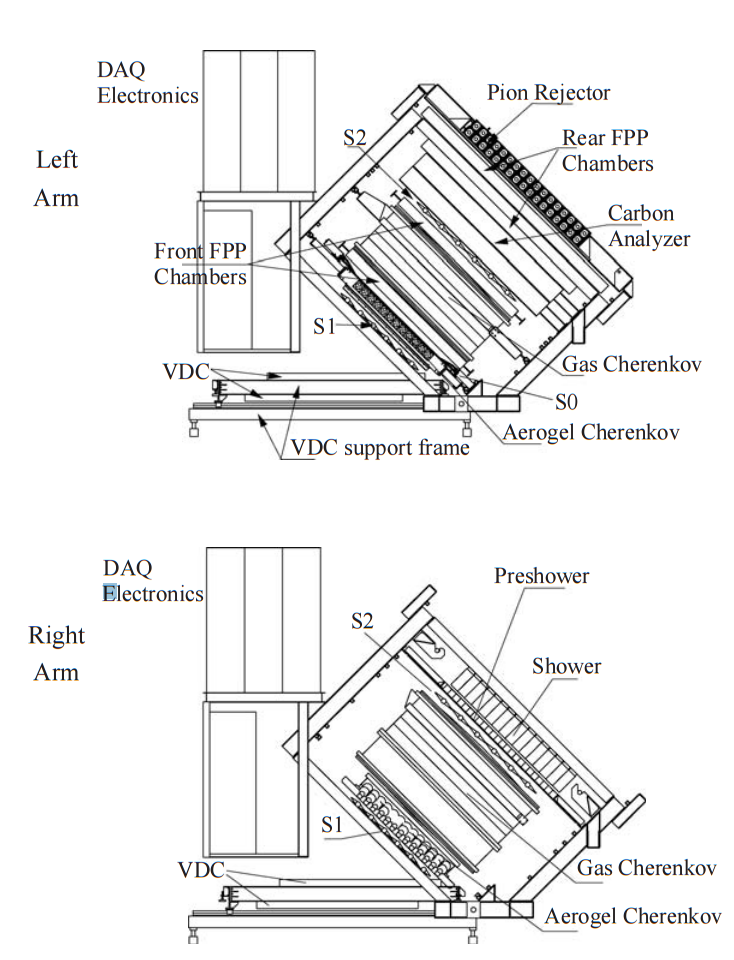
\includegraphics[width=10cm]{HRSs.png}

\caption{A view of both the left(top) and right(bottom) detector stacks inside the left and right HRS \cite{HallA}.
\label{hrsss}}
\end{figure}


	\subsection{Vertical Drift Chambers}
	Each of the spectrometers housed in halla contains a vertical drift chamber(VDC). Each VDC contains two planes of crossing sense wires. Shown in figure \ref{VDC_profile}, the two planes of the VDC lie a distance of 0.335m apart \cite{drift}. The lower plane of the VDC is positioned at the approximate focal plane of the HRS and lies in the horizontal plane of the halla coordinate system. The sense wires located in the VDCs cross orthogonally. They are offset by $45^\circ$ in respect to the dispersive and non-dispersive directions. 
	
	\cite{drift}
	
	
	\begin{figure}
	\centering
	
	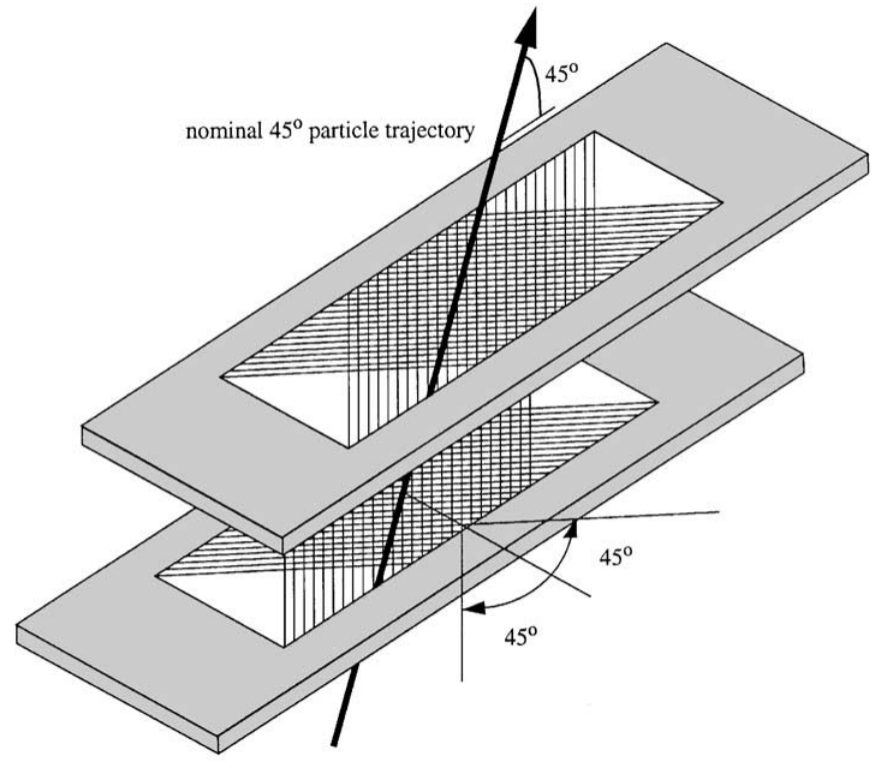
\includegraphics[width=10cm]{VDC_profile_view.png}
	
	\caption{A sketch of the two VDC planes in the HRSs with a particle traveling through the detector at 45$^\circ$.\cite{drift}.
	\label{VDC_profile}}
	\end{figure}
	
	
	
	
	
	\subsection{Scintillators}	\subsection{Cherenkov}
	\subsection{Shower Calorimeter}
	\subsection{Pion Rejector}
	\subsection{FPP Chambers}

\section{Trigger Setup}
\section{DAQ - Data Acquisition System}

\section{Kinematic Settings}









